\chapter{Konzeptionierung}
\label{ch: Konzeptionierung}

In diesem Kapitel wird die Konzeptionierung der Personenerkennung sowie die der Statemachine für das autonome Logistikfahrzeug erläutert. Wie auch in der vorangegangenen Bachelorarbeit geschah die Anforderungserhebung mit der Methode des \textit{Conceptual design specification technique for the engineering of complex Systems} (CONSENS). Am Institut für Systemtechnik der Hochschule Bochum wird zur systematischen Spezifikation von komplexen Systemen die \textit{CONSENS} Methode geschult. Die Anforderungen an die beschriebenen Teilsysteme wurden im Lastenheft als Anforderungsliste ... festgehalten. Die Komponenten für die Entwicklung sind im Umfeldmodell und den entsprechenden Wirkstrukturen dargestellt.
	
	
	\section{Anforderungserhebung mit CONSENS}
	\label{sec: Anforderungserhebung}
	
	In Abbildung \ref{fig: consensenv} ist das erweiterte Umfeldmodell des ALFs zu sehen. Das ursprüngliche Umfeldmodell ist in der entsprechenden Bachelorarbeit wiederzufinden \cite{Bachelorarbeit}. Der Aufbau des Entwurfs besteht im Allgemeinen aus hellblauen und gelben Hexagons, die Wirk- und Umfeldelemente repräsentieren. Der Informationsfluss zwischen den Elementen ist durch gestrichelte Pfeile gekennzeichnet. Das ALF gilt als Kern des Gesamtsystems und ist deswegen im Modell mittig dargestellt. Es interagiert sowohl mit Wirk- als auch mit Umfeldelementen, wie in Abbildung \ref{fig: consensenv} gezeigt. Der Zustandsautomat ist ein Teilsystem, das als Erweiterung des Umfelds gilt. Die von Herrn Dittmann entwickelte kann Sprachverarbeitung sowohl auf dem Rechner des ALFs als auch auf dem integrierten \textit{Raspberry Pi} ausgeführt werden \cite{Dittmann}. Transitionsbedingungen können dementsprechend je nach Anwendungsfall durch beide Hardwarekomponenten intern über das \textit{ROS}-Netzwerk an den EA gesendet.       \\
	
	\begin{figure}[H]
	\begin{center}
		\begin{tikzpicture}
			%\node[CONSENSsys] (env3) at (0,0) {ROS system for manual and autonomous driving};
			\node[CONSENSenv] (env1) at (-7,2) {Kinect\\Sensor(1)};
			\node[CONSENSenv] (env2) at (-7,-2) {Kinect\\Sensor(2)};
			\node[CONSENSsys] (sys1) at (-2,0) {ALF};
			\node[CONSENSsys] (sys2) at (-4,4) {Raspberry\\Pi};
			\node[CONSENSenv] (env3) at (0,4) {Bildschirm};
		%	\node[CONSENSenv] (env4) at (3,-2) {Bildschirm};
			\node[CONSENSenv] (env5) at (0,-4) {Fern-\\bedienung};
			\node[CONSENSenv] (env6) at (-4,-4) {Laut-\\sprecher};
			\node[CONSENSenv] (env8) at (3,0) {Antriebs-\\einheit};
			\node[CONSENSenv] (env7) at (-7,0) {Lidar\\Sensor};
			\node[CONSENSenv] (env9) at (3,2) {Zustands-\\automat};
			
			%27 grad von der ebene
			
			\draw[CSarrow,dashed] (env1.0) -| (sys1.153) node[align = left, font = \scriptsize] at (-4.25,2.4) {Audio Signal,\\Bildinformationen};
			\draw[CSarrow,dashed] (env2.0) -| (sys1.207) node[align = left, font = \scriptsize] at (-4.25,-1.6) {Audio Signal,\\Bildinformationen};
			\draw[CSarrow,dashed] (env7) -- (sys1) node[align = left, font = \scriptsize] at (-4.5,0.4) {Umfeld-\\informationen};
			\draw[CSarrow,dashed] (sys2.0) -| node[above,align=center,font=\scriptsize]{Winkel\\Daten}(sys1.90);
			\draw[CSarrow,dashed] (sys1.58) |- (env3.180) node[align = left, font = \scriptsize] at (-1,3) {Visuali-\\sierung};
			\draw[CSarrow,dashed] (sys1.0) -- node[above,font=\scriptsize]{$4$ x Drehzahlen}(env8.180) ;
			\draw[CSarrow,dashed] (env5.90) |- node[right,align=center,font=\scriptsize]{Benutzer-\\eingaben}(sys1.333);
			\draw[CSarrow,dashed] (sys1.270) |- (env6.0) node[align = left, font = \scriptsize] at (-1,-1.7) {Status-\\informationen};	
			\draw[CSarrow,dashed] (sys1.270) |- (env6.0) node[align = left, font = \scriptsize] at (-1,-1.7) {Status-\\informationen};
			\draw[CSarrow,dashed] (sys1.40) |- (env9.153) node[align = left, font = \scriptsize] at (1.25,3) {Transitions-\\bedingung};
			\draw[CSarrow,dashed] (env9.180) -| (sys1.27) node[align = left, font = \scriptsize] at (-0.4,1.5) {Zustand};
			\draw[CSarrow,dashed] (sys1.122) |- (sys2.333) node[align = left, font = \scriptsize] at (-2.9,2.8) {Audio\\Signal};
			\draw[CSarrow,dashed] (sys2.90) |- (3,5)--(env9.90) node[align = left, font = \scriptsize] at (0,5.2) {Transitionsbedingung};
			%% legende
			
			\node (rect) at (3,-2.0) [draw,thick,minimum width=4.5cm,minimum height=1.75cm] {};
			\node [CONSENSlegendenv] [minimum width=3.8mm,minimum height=6.35mm] (env4) at (1.25,-1.4) {};
			\node [CONSENSlegendsys] [minimum width=3.8mm,minimum height=6.35mm] (sys4) at (1.25,-2.0) {};
			\draw[CSarrow,dashed] (1.0,-2.6) -- node[right]{\footnotesize \Umbruch{}}(1.6,-2.6);
			\node [align=left,font=\footnotesize] (txt1) at (3.35,-1.4) {Umfeldelement};
			\node [align=left,font=\footnotesize] (txt2) at (3.35,-2.0) {Wirkelement};
			\node [align=left,font=\footnotesize] (txt3) at (3.35,-2.6) {Information};
			

			\end{tikzpicture}
			\caption{Weiterentwickeltes Umfeldmodell des Systems ALF. Hierbei wurde das System um die Umfeldelemente des Zustandsautomaten und der integrierten Lautsprecher erweitert. \cite{Bachelorarbeit}}
			\label{fig: consensenv}
	\end{center}
\end{figure}	
	
	Die Erweiterung um die Peronenerkennung ist in der in Abbildung \ref{fig: consensctrl} gezeigten Wirkstruktur dargestellt. Eine Wirkstruktur repräsentiert den Inhalt eines Wirkelements und dient zum besseren Verständnis komplexer Zusammenhänge. In diesem Fall wird das Wirkelement mit dem Titel ALF aus dem vorangegangenem Umfeldmodell \ref{fig: consensenv} aufgeschlüsselt. Die hier gezeigt Wirkstruktur wurde um die Personenerkennung und die Sprachverarbeitung erweitert. Elemente mit blassen Farben sind für diese Masterarbeit eher unwichtig und werden weiterhin nicht behandelt. Für den Betrieb der Personenerkennung sind die Bildinformationen der integrierten \textit{Kinect}-Kameras notwendig. Als Ausgabe werden zweidimensionale Positionen von erkannten Personen für das Visualisierungsprogramm \textit{RViz} veröffentlicht. Für eine mögliche Interaktion mit anwesenden Personen können Statusinformationen, wie oben links in Abbildung \ref{fig: consensctrl} dargestellt, asugegeben werden. Die Ausgabe der Sprachverarbeitung hat durch die Klassifikation der Sprache einen Einfluss auf den Zustandsautomaten und ist somit für das Projekt relevant. Im Umfeldmodell wird die Klassifikation als Transitionsbedingung interpretiert und ist dort als solche gekennzeichnet. \\
		
	\begin{figure}[H]
\begin{center}
\begin{tikzpicture}
%\node[CONSENSsys] (env3) at (0,0) {ROS system for manual and autonomous driving};
\node[CONSENSsysc] (sys1) at (0,0) {Depthimage\\Laserscan(2)};
\node[CONSENSsysc] (sys2) at (3.5,2) {Laserscan\\Merger};
\node[CONSENSsysc] (sys3) at (3.5,-2) {Hector\\SLAM};
\node[CONSENSsysc] (sys4) at (7,-2) {Map\\Server};
\node[CONSENSsysc] (sys5) at (7,2) {Lokalisierung};
\node[CONSENSsysc] (sys6) at (0,2) {RPLidar};
\node[CONSENSsysc] (sys7) at (0,4) {Depthimage\\Laserscan(1)};
\node[CONSENSsys] (sys8) at (0,6) {Personen-\\erkennung};
\node[CONSENSsys] (sys9) at (0,-2) {Sprach-\\verarbeitung};
\node[CONSENSsysc] (sys10) at (7,6) {RViz};
\node[CONSENSsysc] (sys11) at (10.5,6) {Move Base};
\node[CONSENSsysc] (sys12) at (10.5,4) {RALFMain};

\draw[CSarrowc,dashed] (sys10) -- node[midway,right,align=center,font=\scriptsize]{Initial-\\pose}(sys5);
\draw[CSarrowc,dashed] (sys2) -- (sys5) node[above,font=\scriptsize,align=center] at (4.2,4.5){Zusammen-\\geführte\\Messung};
\draw[CSarrow,dashed] (sys8) -- node[above,font=\scriptsize]{Position der Personen}(sys10);
\draw[CSarrowc,dashed] (sys3) -- (sys4) node[above,align=center,font=\scriptsize] at (5.9,-1.5){Aktuelle\\Karte};
\draw[CSarrowc,dashed] (sys10) -- (sys11) node[above] at (8.75,6){\scriptsize \Umbruch{Zielpose}};
\draw[CSarrowc,dashed] (sys11.153) -- node[above,font=\scriptsize]{Costmap}(sys10.27);
\draw[CSarrowc,dashed] (sys11) -- node[right,font=\scriptsize]{}(sys12);
\draw[CSarrowc,dashed] (sys5.east) -| node[align=center,right,font=\scriptsize]{Ist-Pose\\Partikel-\\filter}(sys12.207);
\draw[CSarrowc,dashed] (sys3.333) -- (4.48,-3) -- (11.5,-3) -- (sys12.333) node[above,font=\scriptsize] at (8,-3){Ist-Pose SLAM};
\draw[CSarrowc,dashed] (7,0) -- (8.6,0) -- (8.6,5.5) -- (sys10.333);
\draw[CSarrowc,dashed] (13,4.5) -- node[above,align=center,font=\scriptsize]{\scriptsize Drehzahl\\\scriptsize Drehmoment}(sys12.27);
\draw[CSarrowc,dashed] (13,3.5) -- node[align=center,above,font=\scriptsize]{Gier-\\winkel}(sys12.333);
\draw[CSarrow,dashed] (sys8.north) -- node[align=center,left,font=\scriptsize]{Status-\\informationen}(0,8);
\draw[CSarrow,dashed] (-2.5,4) -- (sys7) node[align=center,font=\scriptsize] at (-0.8,5){Bild-\\informationen};
\draw[CSarrowc,dashed] (6.02,8) -- node[align=center,left,font=\scriptsize]{Benutzer-\\eingaben}(sys10.153);
\draw[CSarrowc,dashed] (sys10.27) -- node[align=center,left,font=\scriptsize]{Visua-\\lisierung}(7.98,8);
\draw[CSarrow,dashed] (-2.5,0) -- (sys1) node[align=center,font=\scriptsize] at (-1.8,-0.5){Bild-\\informationen};
\draw[CSarrowc,dashed] (-2.5,2) -- (sys6) node[align=center,font=\scriptsize] at (-1.6,2.4){2D\\Laser};
\draw[CSarrowc,dashed] (-2.5,-2) -- (sys9) node[align=center,font=\scriptsize] at (-1.8,-2.5){Audio-\\signal};
\draw[CSarrowc,dashed] (sys9.207) -- (-1,-4) node[align=right,font=\scriptsize] at (-0.5,-3.1){Audio-\\stream};
\draw[CSarrow,dashed] (sys9) -- (0,-4) node[align=center,font=\scriptsize] at (0.5,-3.1){Klassifi-\\kation};
\draw[CSarrowc,dashed] (5.4,-2) -- (5.4,4) -- (6,4) -- (sys10.207);
\draw[CSarrow,dashed] (-1.8,4) -- (-1.8,5.5) -- (sys8.207);
\draw[CSarrow,dashed] (-2,0) -- (-2,6.5) -- (sys8.153);
%\draw[CSarrow,dashed] (sys10.207) -| (5.25,5) -- (5.25,-1.5) -- (sys3.27);
\draw[CSarrowc,dashed] (sys3.27) -| (5.1,-1.5) -- (5.1,5.5) -- (sys10.207) node[above,font=\scriptsize] at (4.8,-1.5){};
\draw[CSarrowc,dashed] (4.6,-1.5) -- (sys3.27);
\draw[CSarrowc,dashed] (sys1.east) -| (sys2.south) node[align=center,above,font=\scriptsize] at (1.8,0){Messung\\hinten};
\draw[CSarrowc,dashed] (sys6.east) -- (sys2.west) node[align=center,above,font=\scriptsize] at (1.8,2){Messung\\Lidar};
\draw[CSarrowc,dashed] (sys7.east) -| (sys2.north) node[align=center,above,font=\scriptsize] at (1.8,4){Messung\\vorne};
\draw[CSarrowc,dashed] (sys4.north) -- node[align=center,left,font=\scriptsize]{Statische\\Karte}(sys5.south);
\node[draw=black!40,circle,fill=black!40,scale=0.4] (S1) at (7,0){};
\node[draw=black!40,circle,fill=black!40,scale=0.4] (S1) at (5.4,-2){};
\node[draw=black,circle,fill=black,scale=0.4] (S1) at (-1.8,4){};
\node[draw=black,circle,fill=black,scale=0.4] (S1) at (-2,0){};
\node[draw=black!40,circle,fill=black!40,scale=0.4] (S1) at (5.1,2){};
\draw[CSarrowc,dashed] (sys9.27) -- (1,-0.7) -- (8.9,-0.7) -- (8.9,5.5) -- (sys11.207) node[above,font=\scriptsize] at (3,-0.8){Zielpose};
\draw[CSarrowc,dashed] (sys9.0) -- (1.75,-2) -- (1.75,-4) node[align=left,right,font=\scriptsize] at (1.75,-3.1){Status-\\informationen};
%\draw[CSarrow,dashed] (-4,1) -| node[above]{\footnotesize \Umbruch{$\vec{x}_{t}$}}(sys2);
%\draw[CSarrow,dashed] (sys3) -- node[above]{\footnotesize \Umbruch{$\vec{M}_{t+1}$}}(4.8,0);
%\draw[CSarrow,dashed] (4.8,-1) -| node[below]{\footnotesize \Umbruch{$\vec{\omega}_{t}$}}(sys3.270);
%\draw[CSarrow,dashed] (-4,-1) -| node[below]{\footnotesize \Umbruch{$\vec{u}_{t+1}$}}(sys1);
\end{tikzpicture}
\caption{Wirkstruktur des ALFs. Die für diese Masterarbeit relevanten Wirkelemente und Informationsflüsse sind deckend dargestellt. Eine blasse Farbgebung deutet auf bereits implementierte Teilsysteme hin, die nicht weiter relevant sind, jedoch für ein besseres Verständnis des Gesamtsystems dienen.}
\label{fig: consensctrl}
\end{center}
\end{figure}
	
	\begin{figure}[H]
\begin{center}
\begin{tikzpicture}
%\node[CONSENSsys] (env3) at (0,0) {ROS system for manual and autonomous driving};
\node[CONSENSsys] (sys1) at (0,0) {KNN Personen-\\erkennung};
\node[CONSENSsys] (sys2) at (3.5,0) {Gesichts-\\erkennung};
\node[CONSENSsys] (sys3) at (7,0) {Datenver-\\arbeitung};
%\node[CONSENSsysc] (sys2) at (3.5,2) {Laserscan\\Merger};
%\node[CONSENSsysc] (sys3) at (3.5,-2) {Hector\\SLAM};
%\node[CONSENSsysc] (sys4) at (7,-2) {Map\\Server};
\node[CONSENSsys] (sys5) at (7,2) {Bestimmung\\d. Position};
\node[CONSENSsys] (sys6) at (0,2) {Bestimmung\\d. Distanz};
%\node[CONSENSsysc] (sys7) at (0,4) {Depthimage\\Laserscan(1)};
%\node[CONSENSsys] (sys8) at (0,6) {Personen-\\erkennung};
%\node[CONSENSsys] (sys9) at (0,-2) {Sprach-\\verarbeitung};
%\node[CONSENSsysc] (sys10) at (7,6) {RViz};
%\node[CONSENSsysc] (sys11) at (10.5,6) {Move Base};
%\node[CONSENSsysc] (sys12) at (10.5,4) {RALFMain};

\draw[CSarrow,dashed] (sys1) -- node[midway,left,align=center,font=\scriptsize]{Begrenzungs-\\rahmen}(sys6);
\draw[CSarrow,dashed] (sys1) -- (sys2) node[align=center,font=\scriptsize,above] at (1.75,0.2){Begrenzungs-\\rahmen\\Person};
\draw[CSarrow,dashed] (sys2) -- (sys3) node[align=center,font=\scriptsize,above] at (5.25,0.2){Begrenzungs-\\rahmen\\Gesicht};
\draw[CSarrow,dashed] (sys6) -- (sys5) node[align=center,font=\scriptsize,above] at (3.5,2){Distanz zur Person};
\draw[CSarrow,dashed] (sys5) -- (sys3) node[align=center,font=\scriptsize,right] at (7,1){Position\\d. Person};
%\draw[CSarrowc,dashed] (sys2) -- (sys5) node[above,font=\scriptsize,align=center] at (4.2,4.5){Zusammen-\\geführte\\Messung};
%\draw[CSarrow,dashed] (sys8) -- node[above,font=\scriptsize]{Position der Personen}(sys10);
%\draw[CSarrowc,dashed] (sys3) -- (sys4) node[above,align=center,font=\scriptsize] at (5.9,-1.5){Aktuelle\\Karte};
%\draw[CSarrowc,dashed] (sys10) -- (sys11) node[above] at (8.75,6){\scriptsize \Umbruch{Zielpose}};
%\draw[CSarrowc,dashed] (sys11.153) -- node[above,font=\scriptsize]{Costmap}(sys10.27);
%\draw[CSarrowc,dashed] (sys11) -- node[right,font=\scriptsize]{}(sys12);
%\draw[CSarrowc,dashed] (sys5.east) -| node[align=center,right,font=\scriptsize]{Ist-Pose\\Partikel-\\filter}(sys12.207);
%\draw[CSarrowc,dashed] (sys3.333) -- (4.48,-3) -- (11.5,-3) -- (sys12.333) node[above,font=\scriptsize] at (8,-3){Ist-Pose SLAM};
%\draw[CSarrowc,dashed] (7,0) -- (8.6,0) -- (8.6,5.5) -- (sys10.333);
%\draw[CSarrowc,dashed] (13,4.5) -- node[above,align=center,font=\scriptsize]{\scriptsize Drehzahl\\\scriptsize Drehmoment}(sys12.27);
%\draw[CSarrowc,dashed] (13,3.5) -- node[align=center,above,font=\scriptsize]{Gier-\\winkel}(sys12.333);
%\draw[CSarrow,dashed] (sys8.north) -- node[align=center,left,font=\scriptsize]{Status-\\informationen}(0,8);
%\draw[CSarrow,dashed] (-2.5,4) -- (sys7) node[align=center,font=\scriptsize] at (-0.8,5){Bild-\\informationen};
%\draw[CSarrowc,dashed] (6.02,8) -- node[align=center,left,font=\scriptsize]{Benutzer-\\eingaben}(sys10.153);
%\draw[CSarrowc,dashed] (sys10.27) -- node[align=center,left,font=\scriptsize]{Visua-\\lisierung}(7.98,8);
%\draw[CSarrow,dashed] (-2.5,0) -- (sys1) node[align=center,font=\scriptsize] at (-1.8,-0.5){Bild-\\informationen};
%\draw[CSarrowc,dashed] (-2.5,2) -- (sys6) node[align=center,font=\scriptsize] at (-1.6,2.4){2D\\Laser};
%\draw[CSarrowc,dashed] (-2.5,-2) -- (sys9) node[align=center,font=\scriptsize] at (-1.8,-2.5){Audio-\\signal};
%\draw[CSarrowc,dashed] (sys9.207) -- (-1,-4) node[align=right,font=\scriptsize] at (-0.5,-3.1){Audio-\\stream};
%\draw[CSarrow,dashed] (sys9) -- (0,-4) node[align=center,font=\scriptsize] at (0.5,-3.1){Klassifi-\\kation};
%\draw[CSarrowc,dashed] (5.4,-2) -- (5.4,4) -- (6,4) -- (sys10.207);
%\draw[CSarrow,dashed] (-1.8,4) -- (-1.8,5.5) -- (sys8.207);
%\draw[CSarrow,dashed] (-2,0) -- (-2,6.5) -- (sys8.153);
%%\draw[CSarrow,dashed] (sys10.207) -| (5.25,5) -- (5.25,-1.5) -- (sys3.27);
%\draw[CSarrowc,dashed] (sys3.27) -| (5.1,-1.5) -- (5.1,5.5) -- (sys10.207) node[above,font=\scriptsize] at (4.8,-1.5){};
%\draw[CSarrowc,dashed] (4.6,-1.5) -- (sys3.27);
%\draw[CSarrowc,dashed] (sys1.east) -| (sys2.south) node[align=center,above,font=\scriptsize] at (1.8,0){Messung\\hinten};
%\draw[CSarrowc,dashed] (sys6.east) -- (sys2.west) node[align=center,above,font=\scriptsize] at (1.8,2){Messung\\Lidar};
%\draw[CSarrowc,dashed] (sys7.east) -| (sys2.north) node[align=center,above,font=\scriptsize] at (1.8,4){Messung\\vorne};
%\draw[CSarrowc,dashed] (sys4.north) -- node[align=center,left,font=\scriptsize]{Statische\\Karte}(sys5.south);
%\node[draw=black!40,circle,fill=black!40,scale=0.4] (S1) at (7,0){};
%\node[draw=black!40,circle,fill=black!40,scale=0.4] (S1) at (5.4,-2){};
%\node[draw=black,circle,fill=black,scale=0.4] (S1) at (-1.8,4){};
%\node[draw=black,circle,fill=black,scale=0.4] (S1) at (-2,0){};
%\node[draw=black!40,circle,fill=black!40,scale=0.4] (S1) at (5.1,2){};
%\draw[CSarrowc,dashed] (sys9.27) -- (1,-0.7) -- (8.9,-0.7) -- (8.9,5.5) -- (sys11.207) node[above,font=\scriptsize] at (3,-0.8){Zielpose};
%\draw[CSarrowc,dashed] (sys9.0) -- (1.75,-2) -- (1.75,-4) node[align=left,right,font=\scriptsize] at (1.75,-3.1){Status-\\informationen};
%\draw[CSarrow,dashed] (-4,1) -| node[above]{\footnotesize \Umbruch{$\vec{x}_{t}$}}(sys2);
%\draw[CSarrow,dashed] (sys3) -- node[above]{\footnotesize \Umbruch{$\vec{M}_{t+1}$}}(4.8,0);
%\draw[CSarrow,dashed] (4.8,-1) -| node[below]{\footnotesize \Umbruch{$\vec{\omega}_{t}$}}(sys3.270);
%\draw[CSarrow,dashed] (-4,-1) -| node[below]{\footnotesize \Umbruch{$\vec{u}_{t+1}$}}(sys1);
\end{tikzpicture}
\caption{The system model of the ALV motion control structure. The input of this control is shown on left of this figure. On the right hand sight, the output torque $\vec{M}_{t+1}$ of the described system is illustrated.}
\label{fig: consensctrl}
\end{center}
\end{figure}
	
	\section{Konzept und Aufbau der Personenerkennung}
	\label{sec: Konzept Personenerkennung}
	
	
		\subsection{Wirkstruktur der Personenerkennung}
		
		\subsection{Auswahl und Training der verwendeten neuronalen Netze}
		
		Im diesem Kapitel werden Vergleiche zwischen den in Kapitel \ref{subsec: Objekterkennung durch neuronale Netze} genannten künstlichen neuronalen Netzen gezogen. Weiterhin wird eine Auswahl für die praktische Anwendung am ALF getroffen. 
		
		\begin{table}[htbp]
	\caption{Default Table}
	\label{Tab:SRNRValues}
	\begin{center}
		\begin{tabular}{|c|c|c|c|c|}
			\hline
			\multirow{2}{1.5cm}{Eigen-schaften}& \multicolumn{4}{p{5cm}|}{\centering Netze} \\
			\cline{2-5} & \multicolumn{1}{c|}{VGG-16} & \multicolumn{1}{c|}{ResNet} & \multicolumn{1}{c|}{Inecption} & \multicolumn{1}{c|}{MobileNet} \\ \hline
			Parameter & 27.54 & 13.23 & 6.80 & 6.80 \\
			Eingabe & 29.55 & 9.61 & 6 & 6.80 \\
			Top-5 error & 25.99 & 11.49 & 6.15 & 6.80 \\
			\hline
		\end{tabular}
	\end{center}
\end{table}	
		
		Hinsichtlich der genannten Aspekte wird im Zuge dieser Arbeit ein KNN mit der MobileNet Architektur und dem \textit{Single Shot Detector} (SSD) Framwork verwendet. Die Grundlage der Auswahl wird mithilfe der Paper \textit{MobileNets: Efficient Convolutional Neural Networks for Mobile Vision Applications} \cite{mobilenets} und \textit{The Implementation of CNN-based Object Detector on ARM Embedded Platforms} \cite{embedded} begründet.\\
		
		Die \textit{MobileNet} Architektur ermöglicht im Vergleich zu anderen Lösung zur Merkmalsextraktion den gesuchten Spagat zwischen Schnelligkeit, Genauigkeit und Größe des Netzes \cite{mobilenets}. Das Hauptmerkmal ist der Aufbau der Konvolutionsschichten, der zu den genannten Eigenschaften in der Praxis führt \cite{mobilenets} \cite{embedded}. Vergleichsmessungen zu anderen Architekturen werden in den erwähnten Paper durchgeführt. Der \textit{Single Shot Detector} dient als Klassifikator und zeichnet sich besonders durch seine Schnelligkeit aus \cite{ssd}. Er erreicht eine höhere Genauigkeit als andere state-of-the-art Lösungen wie zum Beispiel \textit{Faster R-CNN} \cite{fasterrcnn} und ist zudem dreimal schneller\cite{ssd}.
		
		\subsection{Entwickeltes neuronales Netz}
		\tikzset{%
			every neuron/.style={
				circle,
				draw,
				minimum size=1cm
			},
			neuron missing/.style={
				draw=none, 
				%scale=4,
				%rotate=90,
				%yshift=1,
				%text height=0.333cm,
				%execute at begin node=\color{black}$\cdots$
			},
		}
		\begin{figure}[H]
			\centering
				
				
				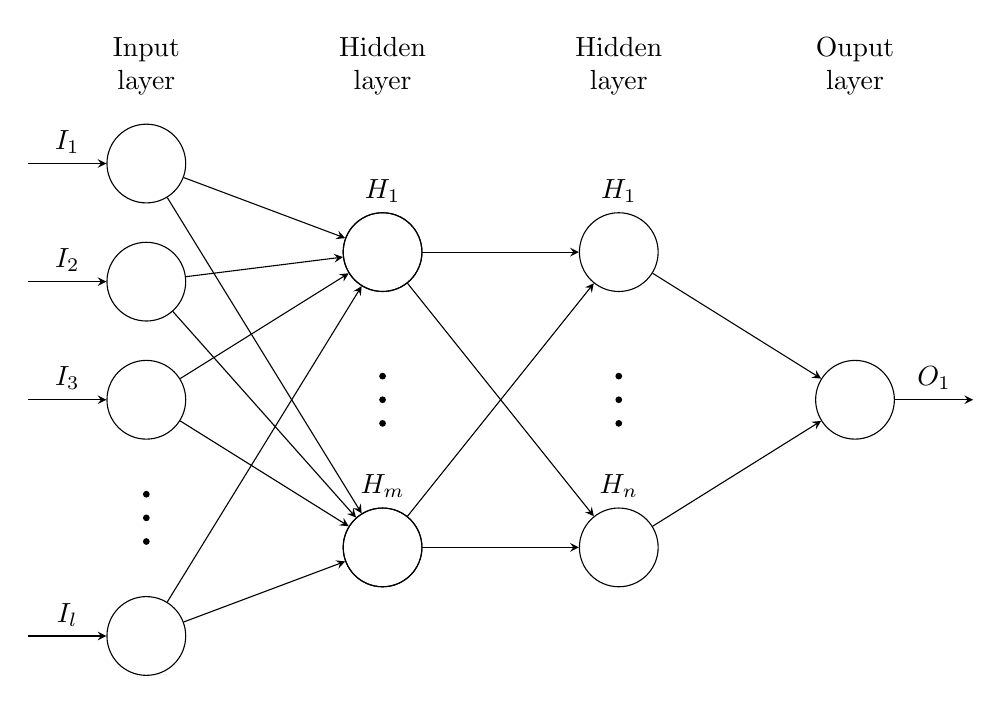
\begin{tikzpicture}[x=1.5cm, y=1.5cm, >=stealth]
					
					\foreach \m/\l [count=\y] in {1,2,3,missing,4}
					\node [every neuron/.try, neuron \m/.try] (input-\m) at (0,2.5-\y) {};
					
					\foreach \m [count=\y] in {1,missing,2}
					\node [every neuron/.try, neuron \m/.try ] (hidden1-\m) at (2,2-\y*1.25) {};
					
					\foreach \m [count=\y] in {1,missing,2}
					\node [every neuron/.try, neuron \m/.try ] (hidden1-\m) at (2,2-\y*1.25) {};
					
					\foreach \m [count=\y] in {1,missing,2}
					\node [every neuron/.try, neuron \m/.try ] (hidden2-\m) at (4,2-\y*1.25) {};
					
					\foreach \m [count=\y] in {1}
					\node [every neuron/.try, neuron \m/.try ] (output-\m) at (6,0.5-\y) {};
					
					\foreach \l [count=\i] in {1,2,3,l}
					\draw [<-] (input-\i) -- ++(-1,0)
					node [above, midway] {$I_\l$};
					
					\foreach \l [count=\i] in {1,m}
					\node [above] at (hidden1-\i.north) {$H_\l$};
					
					\foreach \l [count=\i] in {1,n}
					\node [above] at (hidden2-\i.north) {$H_\l$};
					
					\foreach \l [count=\i] in {1}
					\draw [->] (output-\i) -- ++(1,0)
					node [above, midway] {$O_\l$};
					
					\foreach \i in {1,...,4}
					\foreach \j in {1,...,2}
					\draw [->] (input-\i) -- (hidden1-\j);
					
					\foreach \i in {1,...,2}
					\foreach \j in {1,...,2}
					\draw [->] (hidden1-\i) -- (hidden2-\j);
					
					\foreach \i in {1,...,2}
					\foreach \j in {1}
					\draw [->] (hidden2-\i) -- (output-\j);
					
					\foreach \l [count=\x from 0] in {Input, Hidden, Hidden, Ouput}
					\node [align=center, above] at (\x*2,2) {\l \\ layer};
					\draw[fill=black](0,-1.3)circle(1pt);
					\draw[fill=black](0,-1.5)circle(1pt);
					\draw[fill=black](0,-1.7)circle(1pt);
					\draw[fill=black](2,-0.3)circle(1pt);
					\draw[fill=black](2,-0.5)circle(1pt);
					\draw[fill=black](2,-0.7)circle(1pt);
					\draw[fill=black](4,-0.3)circle(1pt);
					\draw[fill=black](4,-0.5)circle(1pt);
					\draw[fill=black](4,-0.7)circle(1pt);
					
				\end{tikzpicture}
		
		\caption{https://tex.stackexchange.com/questions/132444/diagram-of-an-artificial-neural-network}
		\end{figure}
		\subsection{Schnittstelle zwischen Python und ROS}
		
		\subsection{Erstellung von Objektinformationen}
		\label{subsec: Erstellung von Objektinformationen}
	
	\section{Funktionsweise des Gesamtsystems}
	Der Kern dieser Arbeit ist die Personenerkennung im praktischen Kontext des im Kapitel ... beschriebenen autonomen Logistikfahrzeugs. Aufgrund dessen sind einzelne Programme nicht als abgeschlossenes System zu betrachten. In Kapitel .../consens wurden bereits alle Schnittstellen zu verbauten Hardware- und Softwarekomponenten präsentiert. Das vollständige System der Personenerkennung und der Aufbau des entwickelten, endlichen Automats wird im folgenden Kapitel erklärt.\\
	
	Die Personenerkennung am ALF wird mithilfe der Bildinformationen von zwei \textit{Kinect}-Kameras betrieben. In Kapitel.../rospython wurden bereits zwei Lösungsansätze in der Softwarentwicklung in Zusammenspiel mit ROS und Python präsentiert. Aufgrund einer starken Belastung der im Roboter verbauten Recheneinheit während der parallelen Bildverarbeitung beider eingehender Bilder, wurde das Programm auf eine serielle Verarbeitung umgestellt. Der Befehl der parallelen Verarbeitung erzwingt Berechnungsprozesse mit derselben Frequenz, die durch den Eingang der Bilder beider Kameras vorgegeben wird. Mithilfe der seriellen Abarbeitung  war es ebenfalls möglich die Häufigkeit der Berechnungen zu steuern und damit verbundene Programmoptimierungen vorzunehmen. Auslastungen des verbauten Computers können so eingespart werden und für weitere, parallel laufende Prozesse genutzt werden. Dies wird zum Beispiel durch eine gezielte Verzögerung der Personenerkennung erreicht. Hierbei werden Pausen mit der gewünschten Dauer zwischen Bildverarbeitungsprozessen eingelegt bis ein relevantes Bild erkannt wird. Erst dann arbeitet die Personenerkennung mit der maximalen Geschwindigkeit. Als relevant werden Bilder eingestuft, die eine Person enthalten.\\
	
	\begin{figure}[H]
		\centering
		\begin{tikzpicture}
			\node[circle,fill,gray,minimum size=15mm] (head) {};
			\node[rounded corners=2pt,minimum height=5cm,gray,minimum width=1.5cm,fill,below = 1pt of head] (body) {};
			\draw[line width=3.8mm,gray,round cap-round cap] ([shift={(6pt,-1pt)}]body.north east) --++(-90:19mm);
			\draw[line width=3.8mm,gray,round cap-round cap] ([shift={(-6pt,-1pt)}]body.north west)--++(-90:19mm);
			\draw[thick,white,-round cap] (body.south) --++(90:18mm);
			\node at (0,-2.5) [thick,dashed,rectangle,minimum height=7cm,minimum width=4cm,draw] (v100) {};
			\node at (0,-0.6) [thick,dashdotted,rectangle,minimum height=3cm,minimum width=3.8cm,draw] (v100) {};
			\node at (0,-0.0) [thick,rectangle,minimum height=1.6cm,minimum width=1.6cm,draw] (v100) {};
			
		\end{tikzpicture}
		\caption{test}
		\label{fig: bbox}
	\end{figure}

	In Abbildung \ref{fig: bbox} wird der Ablauf der Personenerkennung in Form eines Programmablaufplans dargestellt. Die Darstellung zeigt die Funktionsweise des Programms ab dem Zeitpunkt, an dem eine Person vor der jeweiligen Kamera detektiert wird. Weiterhin zeigt die Abbildung den Informationsfluss eines Bildes von einer Kamera durch die Personenerkennung. Zu Beginn der Analyse gelangt jedes Bild zunächst in das eingestellte künstliche neuronale Netz. Je nach Anzahl der erkannten Person werden korrespondierende Koordinaten ausgegeben, die die Position des Interessensbereich beschreiben. Anhand dieser Informationen kann an eine Aussage darüber getroffen werden, ob eine Person im Bild zu sehen ist und wo sich diese befindet. Wird keine Person erkannt arbeitet das Programm wieder reduziert, wie bereits beschrieben. Sollten jedoch Personen erkannt worden sein, wird versucht ein Gesicht zu erkennen. In den meisten Fällen sitzen und stehen Menschen aufrecht. So kann davon ausgegangen werden, dass sich das Gesicht einer Person im oberen Teil des Bereichs befindet. Dafür wird der Interessensbereich verkleinert, um Rechenkapazitäten einzusparen. Sollte sich kein Gesicht im relevanten Bereich befinden, wird davon ausgegangen, dass die Person stark von der Kamera abgewandt ist. Somit ist keine eindeutige Identifikation möglich und das Programm schaltet in den reduzierten Modus. Detektiert das Netz ein Gesicht wird eine Merkmalsextraktion durchgeführt.\\
	
	Im Anschluss werden die extrahierten Merkmale mit den der bereits abgespeicherten Gesichtern verglichen. Wird kein übereinstimmendes Gesicht gefunden versucht die Software das Gesicht zu registrieren. Je nach Einstellung wird ein Gesicht registriert, wenn es entsprechend oft hintereinander erkannt worden ist. Der Registrierungsprozess und die Sammlung von Bildinformationen wird in Kapitel \ref{subsec: Erstellung von Objektinformationen} behandelt. Im Falle der Erkennung eines bekannten Gesichts wird die Informationen der erkannten Person wie im bereits erwähnten Kapitel aktualisiert.\\ 
	
	  
	\newpage
	\begin{figure}[H]
		\centering
		\begin{tikzpicture}[node distance = 2cm, auto]
			
			% Place nodes
			\node [papStart] (Start1){Start};
			\node [papProcess, below of = Start1,label={[shift={(5,-0.6)}]\footnotesize\textit{Aktuelles Bild wird mit KNN analysiert}}] (pro1){Prozess};
			\node [papDecision, below of = pro1, yshift= -9mm,label={[shift={(2.7,-0.6)}]\footnotesize\textit{Menschen im Bild?}}](dec1){Entscheidung};
			\node [papProcess, right of = dec1,xshift=25mm,label={[shift={(5,-0.6)}]\footnotesize\textit{Gesichter im Interessensbereich detektieren}}](pro3){Prozess};
			\node [papDecision, below of = pro3, yshift= -9mm,label={[shift={(5,-0.6)}]\footnotesize\textit{Gesicht im Interessenbereich?}}](dec2){Entscheidung};
			\node [papProcess, below of = dec2, yshift= -9mm,label={[shift={(5,-0.6)}]\footnotesize\textit{Merkmalsextraktion des Gesichts}}](pro4){Prozess};
			\node [papDecision, below of = pro4, yshift= -9mm,label={[shift={(5,-0.6)}]\footnotesize\textit{Gesicht bekannt?}}](dec3){Entscheidung};
			\node [papDecision, below of = dec3, yshift= -18mm,label={[shift={(5,-0.6)}]\footnotesize\textit{Dasselbe unbekannte Gesicht oft genug hintereinander erkannt?}}](dec4){Entscheidung};
			\node [papProcess, below of = dec4, yshift= -9mm,label={[shift={(5,-0.6)}]\footnotesize\textit{Eigenschaften des Objekts vom Typ Mensch aktualisieren}}](pro5){Prozess};
			%\node [papData, right of = dec3, xshift= 25mm,label={[shift={(5,-0.6)}]\footnotesize\textit{Gesicht bekannt?}}](dat1){I/O};
			\node [papEnd, below of = dec1, yshift= -40mm] (End) {Ende};
			
			% Place joins
			\coordinate [below of = dec1, yshift= -9mm] (join1);
			
			% Draw edges
			\path [papLine] (Start1) -- (pro1);
			\path [papLine] (pro1) -- (dec1);
			\path [papLine] (dec1) -- node [above] {\papYes} (pro3);
			\draw (dec1) -- node [right] {\papNo} (join1);
			\path [papLine] (pro3) -- (dec2);
		%	\path [papLine] (dec2) -- node [above] {\papYes} (pro4)
			\draw (dec2) -- node [above] {\papNo} (join1);
			
			\path [papLine] (join1) -- (End);
			
		\end{tikzpicture}
		\label{fig: Personenerkennung}
	\end{figure}
	
	\section{Umsetzung der Statemachine}
	\label{sec: Umsetzung der Statemachine}
	Für die Steuerung des autonomen Logistikfahrzeugs durch eine Spracherkennung wurde ein endlicher Automat entwickelt. Die Entwicklung der Spracherkennung wird in der Masterarbeit von Hannes Dittmann erläutert. In der vorangegangenen Bachelorarbeit werden die Fahrfunktionen des Roboters erklärt. Der Grundgedanke und die daraus resultierende Auswahl des Zustandsautomats wird im folgendem Kapitel näher ausgeführt.\\	
	
		\subsection{Auslegung des Zustandsautomats}
		Die Problematik der Steuerung über Sprache ist die Extraktion der eigentlichen Aussage eines Satzes. In der Masterarbeit von Hannes Dittmann werden aufgrund dessen Sprachbefehle kategorisiert. Die KI ist in der Lage verschiedene Sätze einer für den Roboter relevanten Kategorie zuzuordnen. Diese werden als Eingabeparameter für den EA genutzt. Weiterhin wird zwischen einer manuellen und einer autonomen Fahraufgabe unterschieden und als zweiten Parameter für den Zustandsautomaten genutzt. Anhand der technischen Fähigkeiten des Roboters wurden die Kategorienamen so gewählt, dass alle möglichen Handlungen abgedeckt sind. Der Zustandsautomat wurde so entworfen, dass er trotz der vielen Handlungsmöglichkeiten des Roboters mit möglichst wenig Zuständen arbeitet. Für die größtmögliche Effizienz hinsichtlich der Dimension des EAs wurde ein mathematisches Modell entworfen.\\
		
		\begin{equation}
			\vec{z}=\sum_{z=0}^{z_f} \left[ \begin{array}{r}
				k_n  \\
				k_{n+1}  \\
				.  \\
				.  \\
			\end{array}\right] \circ
			\left[ \begin{array}{r}
				b_n(z)  \\
				b_{n+1}(z)  \\
				.  \\
				.  \\
			\end{array}\right]  \circ
			\left[ \begin{array}{r}
				1  \\
				1  \\
				l(z_f)  \\
				l(z_f)  \\
				1  \\
				f_m  \\
				f_a  \\
				l(z_f)\cdot f_a  \\
				l(z_f)\cdot f_a \\
			\end{array}\right] 
			\label{eq: statemachine}
		\end{equation}\\
	
		\begin{equation}
			b_n(z)=\left\{\begin{array}{ll} 1 \text{ für } z=n \\
				0 \text{ für }z\neq n\end{array}\right. .
			\label{eq: Binärfunktion}
		\end{equation}\\
	
		Dies ermöglicht einen sich aufbauenden Endzustand in Form eines Zustandsvektors $\vec{z}$ und wird im folgenden Beispiel anhand der Gleichung \ref{eq: statemachine} und \ref{eq: Binärfunktion} erläutert. Es wird angenommen, dass der Endzustand $z_f=6$ erreicht werden soll. Der sechste, finale Zustand ist die manuelle Steuerung des Roboters über den Controller. Durch die Variable $z$ werden Zustände beschrieben, die vor Erreichen des Endzustands durchlaufen werden müssen. Jeder Zustand $z$ verfügt über eine eigene Knotenmenge $k_n$, die in Form von ROS-Knoten aufgerufen werden. Die Hilfssunktion $b_n(z)$ ist eine binäre Funktion und aktiviert im jeweiligen Index der Summe die benötige Knotenmenge $k_n$
	
		
		
		
		In diesem Zusammenhang kam während der Entwicklung die Idee einer Fusion der Personen- und Spracherkennung in der Praxis auf.  
		
	
		
		
				   		

